% Mirror: https://github.com/SIGma-UIUC/presentation-format
% --------------------------------------------------------------------
% This is a simple Beamer document that uses beamerthemesigma.sty
% Reading the comments should help you create a presentation even if
% you've never used Beamer before.
% --------------------------------------------------------------------

% Set our document class to Beamer
\documentclass[handout, aspectratio=169]{beamer}
% \documentclass[aspectratio=169, handout]{beamer}
% Add handout option to ignore pauses

% From Jeff E
\usepackage{algo}
% Some more macros
\usepackage{sigmastyle}

\usepackage{gensymb}

\usepackage{amsmath}
\usepackage{amssymb}


% Set a title
\title{Shor's Algorithm}

% Set a subtitle if you desire

% Whoever worked on the presentation:
\author{Andrey Vlasov}

% Date looks ugly, so leave blank
\date{}
\newcommand{\twovec}[2]{\begin{pmatrix} #1 \\ #2 \end{pmatrix}}
\newcommand{\tworvec}[2]{\begin{pmatrix} #1 & #2 \end{pmatrix}}
\newcommand{\twomat}[4]{\begin{pmatrix} #1 & #2 \\ #3 & #4 \end{pmatrix}}

% An institute name, if you're so inclined
% \institute{University of Illinois Urbana-Champaign}

% Use the SIGma theme for this Beamer presentation
\usetheme{sigma}
% --------------------------------------------------------------------

% Begin document
\begin{document}

% Beamer calls each slide a "frame", defined within the environment:
% \begin{frame}
%   <frame content here>
% \end{frame}

% This frame is just the title.
\begin{frame}
\titlepage
\end{frame}

% A frame with the table of contents.
% This frame's title is "Outline".
\begin{frame}{Outline}
  \tableofcontents
\end{frame}

\section{The RSA problem}
\frame{\sectionpage}
\begin{frame}{The RSA problem}
    \begin{itemize}
        \item Given the public keys $N$ and $e$, and the publicly transmitted ciphertext $C\equiv M^e\pmod N$, find the original message $M$. \pause
        \item Currently an open problem, but it's believed that factoring $N$ is the best approach. \pause
        \item Factoring $N$ will also give us the private key $d$, so we can decode any messages sent with this key pair. \pause
        \item Thus, our problem becomes: Given a semiprime $N=pq$, find the prime factors $p$ and $q$ of $N$. \pause
    \end{itemize}
\end{frame}

\section{Shor's algorithm}
\frame{\sectionpage}

\begin{frame}{A definition}
    \begin{itemize}
        \item Let $a$ and $N$ be integers such that $a$ is \textcolor{sigma@mainblue}{coprime to $N$}. \pause
        \item The order of $a\pmod N$ is the \textcolor{sigma@mainblue}{smallest} positive integer $r$ such that $a^r\equiv 1\pmod N$. \pause
        \item By Euler's Theorem, $a^{\phi(N)}\equiv 1\pmod N$. Thus, $r|\phi(N)$. \pause
        \item In Shor's algorithm, the problem of factoring $N$ is replaced with the problem of finding $r$.
    \end{itemize}
\end{frame}

\begin{frame}{Step 1: RNG}
    \begin{itemize}
        \item Pick a random number $a$ with $1<a<N$, and calculate $\gcd(a, N)$. \pause
        \item If $\gcd(a, N)\not=1$, we got really lucky. Since $N$ has only two factors, $p=\gcd(a,N)$ and $q=N/p$. \pause
        \item If $\gcd(a,N)=1$, we move on to step 2.
    \end{itemize}
\end{frame}

\begin{frame}{Step 2: Order-Finding}
    \begin{itemize}
        \item Find the multiplicative order of $a\pmod N$ and label it $r$. \pause
        \item $a^r\equiv 1\pmod N$ \pause $\Rightarrow\ N|(a^r-1)$ \pause $\Rightarrow\ N|(a^\frac{r}{2}-1)(a^\frac{r}{2}+1)$ \pause
        \item If $r$ is odd, we can't use this formula, so we go back to step 1. \pause
        \item It's impossible that $N|(a^\frac{r}{2}-1)$, because then $a^\frac{r}{2}\equiv 1\pmod N$, but the order of $a\pmod N$ is $r>\frac{r}{2}$. \pause
        \item Ideally, $N$ shares a factor with $(a^\frac{r}{2}-1)$ that's less than $N$.
    \end{itemize}
\end{frame}

\begin{frame}{Step 3: Factor}
    \begin{itemize}
        \item Compute $g=\gcd(N, a^\frac{r}{2}-1)$. \pause
        \item If $g=1$, then $N|(a^\frac{r}{2}+1)$, which tells us nothing about the factors of $N$. So, we go back to step 1. \pause
        \item If $g>1$, then $g$ is one of the prime factors of $N$, and the other factor is $N/g$. \pause
        \item In his original paper, Shor proved that the probability of the algorithm working, given a random $a$, is at least $\frac{1}{2}$. The exact probability is an open problem!
    \end{itemize}
\end{frame}

\section{Implementing the algorithm}
\frame{\sectionpage}

\begin{frame}{Classical part}
    \begin{itemize}
        \item A classical computer is used for steps 1 and 3, because it can calculate the $\gcd$ of two numbers very quickly. \pause
        \item In fact, this calculation never needs more steps than 5 times the number of digits!
    \end{itemize}
\end{frame}

\begin{frame}{Proof of $\gcd$ complexity}
    \begin{itemize}
        \item Claim: Worst-case for Euclidean algorithm is two Fibonacci numbers \pause
        \item More specifically, if the algorithm requires $N$ steps to find $\gcd(a,b)$ with $a>b$, then $a\geq F_{N+2}$ and $b\geq F_{N+1}$ \pause
        \item Base case: $N=1$. The smallest pair is $a=2=F_3$ and $b=1=F_2$ \pause
        \item Inductive step: Assume claim is true for all $N\leq K-1$ \pause
        \item The first step in an algorithm with $K$ steps is $a=qb+r$. Consider the pair $b$ and $r$ ($b>r$), which takes $K-1$ steps \pause
        \item By the inductive hypothesis, $b\geq F_{K+1}$ and $r\geq F_{K}$ \pause
        \item $a=qb+r\geq b+r\geq F_{K+1}+F_K=F_{K+2}$
    \end{itemize}
\end{frame}

\begin{frame}{Proof of $\gcd$ complexity}
    \begin{itemize}
        \item A property of the golden ratio: $\phi^2=\phi+1$ \pause
        \item This gives a property of Fibonacci numbers: $\phi^N=\phi F_N+F_{N-1}$ \pause
        \item $\phi^N=\phi F_N+F_{N-1}\leq \phi F_N+F_N=(\phi+1)F_N=\phi^2 F_N$
        \item $\phi^{N-2}\leq F_N$ \pause
    \end{itemize}
\end{frame}

\begin{frame}{Proof of $\gcd$ complexity}
    \begin{itemize}
        \item If the Euclidean algorithm takes $N-1$ steps, then $b\geq F_N\geq \phi^{N-2}$ \pause
        \item $N-2\leq \log_\phi(b)$ and $\log_{10}(\phi)>\frac{1}{5}$, so
        \begin{equation*}
            \frac{N-2}{5}\leq \log_{10}(\phi)\log_\phi(b)=\log_{10}(b)
        \end{equation*} \pause
        \begin{equation*}
            N-1\leq 1+5\log_{10}(b)<5\log_{10}(b)
        \end{equation*} \pause
        \item Time complexity is $O(\log(b))$ - only depends on the smaller number!
    \end{itemize}
\end{frame}

\begin{frame}{Quantum part}
    \begin{itemize}
        \item Finding the order of a number is hard for classical computers. \pause
        \item The best known algorithm (repeated squaring) is subexponential. \pause
        \item So, we plug the output from step 1 into a quantum computer. \pause
        \item The quantum circuit complexity is $O(n^3)$ - much better!
    \end{itemize}
\end{frame}

\section{So why isn't RSA broken?}
\frame{\sectionpage}

\begin{frame}{So why isn't RSA broken?}
    \begin{itemize}
        \item Shor's algorithm needs perfect qubits, with no errors. \pause
        \item In real quantum systems, errors are really hard to correct. \\
        (see meetings 3 and 4 from Fall '23) \pause
        \item Order-finding algorithm requires $2n+3$ qubits for an $n$-bit number. \pause
        \item For 2048-bit RSA, would need 4,099 perfect qubits. \pause
        \item Current best: IBM's Condor with 1,121 noisy qubits.
    \end{itemize}
\end{frame}

% Asking questions is fun but we should answer some first
\begin{frame}{}
      \begin{center}
    {\color{sigma@mainblue} \LARGE Questions?}
  \end{center}
\end{frame}

\begin{frame}{Relevant xkcd}
  \begin{figure}
      \centering
      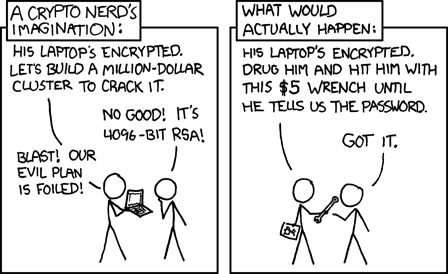
\includegraphics[scale=0.65]{xkcd_rsa.png}
  \end{figure}
\end{frame}

% Remove this slide if you came up with all the material yourself
\begin{frame}{Bibliography}
    \nocite{Wong}
    \nocite{Shor}
    \bibliography{refs}
    \bibliographystyle{alpha}
\end{frame}

\end{document}